% \setchapterimage[6cm]{seaside}
\setchapterstyle{kao}
\setchapterpreamble[u]{\margintoc}
\chapter{The first large \bcomment{auto-regressive}{incremental (everywhere)} language model for French}
% using a generative objective
\labch{generative}

% \cleanchapterquote{\textup{[\,\dots]} le sujet s’éloigne du verbe et \textup{[\,\dots]} le complément vient se poser quelque part dans le vide.}{Samuel Beckett}{Malone meurt, 1951}
\cleanchapterquote{La nuit se faisait assez obscure, les étoiles semblaient dormir de temps à autre, cependant le peu de clarté qui me permit de marcher la nuit dans la chambre éveilla en moi une profonde pitié de ce que je faisais là, et cette peur de l'avenir me devint plus vive et plus aiguë.}{Automatic text generation}{$\text{GPT}_{fr}$-1B, 2021}

% \section{Training efficient sentence embedding models using structured encoders}
% \labsec{structure-scale}
% Previous sections examined the training of models by predicting relationships between sentences. Here, 

\acomment{The previous section discussed enhancing large transformer language models using self-supervised objectives adapted for sentence embeddings. Our procedure reached state-of-the-art results on many downstream evaluation tasks. However, we did not perform the initial pre-training ourselves but instead used already pre-trained transformers for English. This section presents a quantitative evaluation of the effort required to pre-train such models in terms of data collection, computing infrastructure configuration, model development, and evaluation. To be as representative as possible of the process, we chose a language and architecture design for which \bcomment{few resources}{french is usually said to be a well resourced language} were available. The section thus relates the pre-training of the first large auto-regressive language model for French \parencite{simoulin_2021c}.

Auto-encoding model have already been developed in French, namely CamemBERT \parencite{martin_20} or FlauBERT \parencite{le_20a, le_20b}. However, to the best of our knowledge, this contribution is the first peer-reviewed to adapt pre-trained auto-regressive transformers to French. In particular, we introduced a French version from the well-known GPT model \parencite{radford_2018, radford_2019, brown_20}. GPT, which stands for Generative Pre-trained Transformer, is an auto-regressive language model developed by Open AI research laboratory\sidenote{\url{https://openai.com/}}. \bert and other models presented in the previous sections act as encoders, taking text as input and producing vector representations as output. On the contrary, GPT acts as a decoder, taking text as input and producing text as output. 
%rappeler ce qu'est GPT, et donner une spécification de ton modèle dans le chapitre, segmentation etc; contraster l'objectif avec celui de BERT etc histoire que le chapitre soit stand alone.
% Parler du défi pour entrainer ce type de model
%\bcomment{titre mal choisi}{Camembert et flaubert sont venus avant}

From a modeling point of view, \gpt is an incremental language model whose pre-training objective is relatively similar to the one from a n-gram language model already used 30 years ago. But while n-gram language models typically use a context size of 5 or fewer words, \gpt extends the context size to \numprint{1024} tokens. From a practical point of view, pre-training such a model is a superlative project, which is far from trivial. First, it requires large corpora of raw text—up to billion of tokens. Second, the analysis and evaluation of these models require access to relevant and rigorous benchmarks. Last but not least, pre-training also requires significant computing power. It requires distributing the training on multiple computing units across multiple computing nodes. Typically dozens of graphics processing unit (GPUs) or tensor processing units (TPUs) %\sidenote{\url{https://cloud.google.com/tpu}} 
operating for several days. In that regard, this work benefited from access to the IDRIS computing facilities through the allocation of 2020-AD011011823 allocated by GENCI. Our model was among the first to be trained on the super-computer Jean-Zay, less than one year after its inauguration in January 2020.} Our contributions are the following:
\begin{itemize}
    \item We propose a corpus dedicated to the training of transformers language models in French. We detail the construction of this corpus in \refsec{generative:corpus} ;
    \item We \acomment{trained} two models with a large number of parameters, which we released as open-source contributions\sidenote{\url{https://huggingface.co/asi/gpt-fr-cased-base}}. Hopefully, these models can be used in academic as well as industrial settings ;
    \item We replicate English evaluation benchmarks for French language models. This evaluation setup allows for the comparison of models and is detailed in \refsec{generative:evaluation}.
\end{itemize}

% We organize the section as follow: We first present the construction of the training and evaluation corpora (\refsec{generative:corpus}). We then detail the architecture and training setup in \refsec{generative:models}. Finally,  \refsec{generative:evaluation} examines our model abilities through several evaluation tests.

% In this case, we are mining a specific datasets with many sentence pairs. \bcomment{There are also methods for reconstructing a noised input, for example detecting masked words or predicting what the next word will be. The corpora required for such auto-encoding methods are more simple and only consist in individual documents.}{raw text ?}

% In this section, we introduce a French \bcomment{adaptation}{version} from the well-known \bcomment{GPT}{rappeler ce qu'est GPT, et donner une spécification de ton modèle dans le chapitre, segmentation etc; contraster l'objectif avec celui de BERT etc histoire que le chapitre soit stand alone} model. GPT relies on transformer pre-trained architectures, which profoundly transformed natural language processing methods. Such models are pre-trained using a self-supervised objective and are therefore specific to a given language. The model, equivalent to GPT-2 in English, contains more than 1 billion parameters. \bcomment{This work benefited from access to the IDRIS computing facilities through the allocation of 2020-AD011011823 allocated by GENCI.}{dire que ce modèle est un des premiers à avoir été entrainé sur l'IDRIS, mettre en avant dans le chapitre le coté infrastructure : calcul distribué, combien de noeuds, temps d'entrainement etc.}

% Although some models may exist in French, the majority is released in \bcomment{English}{cela vaudrait le coup d'inclure une section qui résume un peu ce qui change; est-il aussi facile de trouver les données ? commenter le zero-shot etc.} only.  

\acomment{
We organize the section as follow: \refsec{generative:incremental} first reviews the main characteristic of auto-regressive models, their originality and main distinctions with standard encoders. \refsec{generative:corpus} then presents the constitution of the pre-training corpora. We then detail and training and evaluation procedure in \refsec{generative:training} and \refsec{generative:evaluation}. Finally, we discuss the limits and ethical consideration in \refsec{generative:limits}.
}

%GPT achieves impressive language generation performances. 

% Within my laboratory, I led the project to train the first large language model in French \parencite{simoulin_2021c}. We obtained a dedicated computation grant on public French HPC computer Jean Zay. The model, equivalent to GPT-2 in English, contains more than 1 billion parameters. We built a dedicated training corpus and parallelized the training between multiple nodes and compute units. I am particularly proud of this project, as we contributed to the resources available in French. We released the model in Open-Source for research and business application purposes. 

%TODO il faut parler des embeddings de phrase de ces modèles et le relier à la problématique de la thèse

% This is, to the best of our knowledge, the first peer-reviewed contribution that \bcomment{adapts pre-trained generative transformers}{nope there are camembert and flaubert} to French. We adapt OpenAI GPT et GPT-2 \parencite{radford_2018, radford_2019} for French. Our contributions are the following:
% \begin{itemize}
%     \item We propose a corpus dedicated to the training of transformers language models in French. The construction of thus corpus is detailed in \refsec{generative:corpus} ;
%     \item We \acomment{trained} two models with a large number of parameters, which we released as open-source contributions\sidenote{\url{https://huggingface.co/asi/gpt-fr-cased-base}}. Hopefully, these models can be used in academic as well as industrial settings. We detailed the architecture of the models in \refsec{generative:models} ;
%     \item We replicate English evaluation benchmarks for French language models. This evaluation setup allows for the comparison of models and is detailed in \refsec{generative:evaluation}.
% \end{itemize}

\section{Auto-regressive language models}
\labsec{generative:incremental}
% rappeler ce qu'est GPT, et donner une spécification de ton modèle dans le chapitre, segmentation etc; contraster l'objectif avec celui de BERT etc histoire que le chapitre soit stand alone
% cela vaudrait le coup d'inclure une section qui résume un peu ce qui change; est-il aussi facile de trouver les données ? commenter le zero-shot etc.
% The model can address a large variety of tasks. In particular, the model may benefit from original configurations such as few-shot or zero-shot learning. In such configurations, it is possible to address tasks without any parameters fine-tuning.

% Assuming pre-training corpus consists of a sequence of tokens $U=\{u_1 \cdots u_T\}$, the model can finally be described simply according to the following equations:

\acomment{As detailed in \refsec{architectures:transformers}, \gpt or \bert are based on transformer architectures. Both models take as input sequence of tokens\sidenote{Here we tokenize the input text using bytepair vocabulary encoding (BPE) with \numprint{50000} units \parencite{sennrich_16a}. This procedure allows for a relatively reduced vocabulary size while drastically reducing the number of tokens out of the vocabulary.} and encode them as the sum of a token and positional embeddings (\refeq{generative:embeddings}). Token embedding vectors are then transformed into so-called contextualized vectors through a series of $L$ transformer layers (\refeq{generative:layers-eq}).

\begin{align}
    h^0_t &= W_eu_t + W_p \quad \forall t \in \llbracket 1, T \rrbracket \labeq{generative:embeddings} \\
    h^n_t &= \mathsf{layer}(h^{n-1}_t) \quad \forall n \in \llbracket 1, L \rrbracket \labeq{generative:layers-eq}
\end{align}

With $\{u_1 \cdots u_T\}$ the sequence of input tokens, $L$ the number of layers, $W_e$ the embedding matrix, and $W_p$ the positional embedding matrix.

% \begin{gather}
% \begin{align}
%     & h_0^t = u^tW_e+W_p \labeq{generative:embeddings}\\
%     &h_i = \textrm{decoder\_layer}(h_{i-1}), \quad \forall i \in [1,n] \\
% \end{align}
% \end{gather}

Each layer in \refeq{generative:layers-eq} acts as a many-to-many encoder. \bert and its derivatives use so-called encoder layers: it computes contextualized representations given the right and left contexts \ie from the tokens immediately after and before the considered position. \gpt, however, relies on decoder layers: contextualized representations only depend on the left context, that is, tokens before the considered position. We illustrate this key distinction in \reffig{generative:self-attention-decoder}.}

\begin{figure}[htbp]
\begin{center}
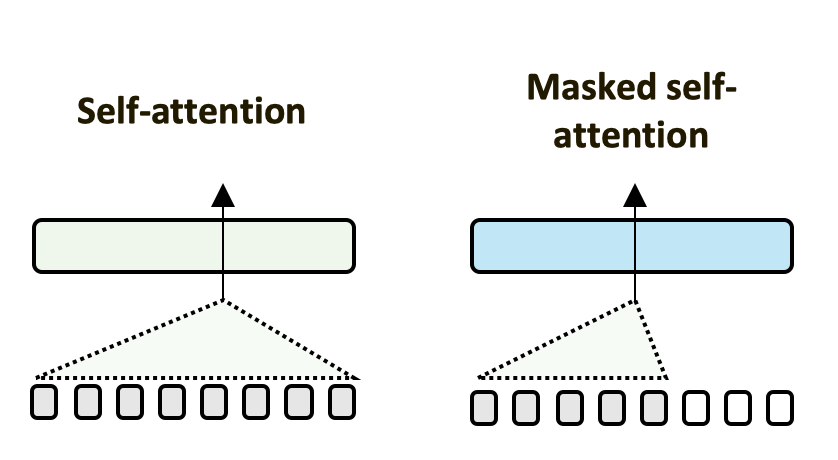
\includegraphics[width=8cm]{images/self-attention.png}
\end{center}
\caption{Illustration of the self-attention scope for encoding and decoding layers.}
\labfig{generative:self-attention-decoder}
\end{figure}

% and \bcomment{shares many similarities with \textsc{Bert}}{too fuzzy, which ones ?}. It consists in successive decoder layers. The main difference with \textsc{Bert} is that the multi attention-heads only focus on tokens preceding the considered position. \bcomment{too fuzzy }{introduce that earlier and with a cleaner formalization}

\acomment{This \bcomment{slight}{pq slight? rm} difference in design has important implications for both architectures' training and inference setups. We detail such implications during the pre-training phase in \refsec{generative:autoregressive:pre-training} and during inference in \refsec{generative:autoregressive:inference}.
}

\subsection{Pre-training}
\labsec{generative:autoregressive:pre-training}

\acomment{\bert and \gpt are pre-trained using a language model training objective: they associate a probability $P(u_1 \cdots u_T)$ to a sequence of tokens. We can decompose this sequence probability as the product of conditional probabilities for each token:

\begin{equation}
    P(u_1 \cdots u_T) = \prod_{t \in \llbracket 1, T \rrbracket} P\left(u_t \middle| U \right)
\end{equation}

With $U$ the context of $u_t, \forall t \in \llbracket 1, T \rrbracket$. Given the contextualized representations of each token from \refeq{generative:layers-eq}, we can compute the conditional probabilities associated with each token given \refeq{generative:token-proba}.

\begin{equation}
    P\left(u_t \middle| U \right) = \textrm{softmax}(h_t^N W_e^T) \labeq{generative:token-proba} \\
    % \mathcal{L}(U) = \sum_i log P\left(u_{i} \middle| u_{i-k} \cdots u_{i-1}  ; \Theta\right)
\end{equation}

With $h_t^N$ the contextualized representation from the last layer of the token at index $t$. 

\bert relies on a bidirectional context to build representations. Each token contextualized representation is conditioned on every other tokens from the input, including himself, such that $P\left(u_t \middle| U \right) = P\left(u_t \middle| u_1 \cdots u_T \right)$. Since, a given token contextualized representation depends on the token itself, \bert uses a \textit{trick} for pre-training by replacing some tokens with a \texttt{[MASK]} in the input text. Thus, such tokens are "masked" and not used to build contextualized representations. The model is then trained to predict the original token at masked positions. 

\gpt only uses the left context to build token representations, such that $P\left(u_t \middle| U \right) = P\left(u_t \middle| u_1 \cdots u_{t-1} \right)$. Therefore, it is unnecessary to use such artifice. We only pre-train the model using a standard incremental language model objective: predicting the next token given the previous ones. Assuming the pre-training corpus $D$ consists of a collection of documents $d=\{u_1 \cdots u_T\}$\sidenote{To simplify the notations, we omit the document index such that we refer to the tokens of all documents as $\{u_1 \cdots u_T\}$ and not $\{u^{(d})_1 \cdots u^{(d)}_T\}$.}, we optimize the \gpt parameters $\Theta$ to maximize the following log-likelihood:% $\mathcal{L}(U)= \sum_i log P\left(u_{i} \middle| u_{i-k} \cdots u_{i-1}  ; \Theta\right)$. 

\begin{equation}
    \mathcal{L}(D) = \sum_{d \in D}\sum_{i \in \llbracket 1, T \rrbracket} \log P\left(u_{i} \middle| u_{i-k} \cdots u_{i-1}  ; \Theta\right)
\end{equation}

With $k$ the context-size, and $U=\{u_{i-k} \cdots u_{i-1}\}$ the context of the token at position $i$.
}

\subsection{Inference}
\labsec{generative:autoregressive:inference}

\acomment{
\paragraph{Standard fine-tuning} Once the model is pre-trained, it is possible to fine-tune it on downstream tasks. Fine-tuning incrementally adjusts all model parameters to optimize the loss on a specific task. In such case, we take tokenized text as input $X = x_1 \cdots x_m$. We transform the input using our transformer into contextualized representations $h^N_1 \cdots x^N_m$ (\refeq{generative:gpt-std}). We then feed representations from the sequence to a dense layer with parameters $W_y$ followed by a softmax to predict the label $\hat{y}$ (\refeq{generative:softmax}). In the case of \bert, we usually use the first token $h^N_1$ of the sequence as input of the dense layer. For \gpt, we usually use the last token $h^N_m$. We seek to optimize a loss function comparing the true labels $y$ with the predictions $\hat{y}$ (\refeq{generative:loss}). 

% P\left(y \middle| x^1 \cdots x^m \right)
\begin{align}
    h_N^m &= \textrm{GPT}(x_1 \cdots x_m) \labeq{generative:gpt-std} \\
    \hat{y} &= \textrm{softmax}(h_N^m W_y) \labeq{generative:softmax} \\
    \mathcal{L} &= \sum_{y \in Y} \mathcal{L}(\hat{y}, y) \labeq{generative:loss} 
\end{align}

On the one hand, when encoding a fixed-length text for downstream tasks, \gpt deprives itself of half of the contextualized information and thus usually reaches performances below \bert on many downstream tasks. On the other hand, since \gpt only uses the left context to build contextualized representations, it is a natural candidate for natural language generation. We illustrate this configuration in \reffig{generative:inference} (right sub-figure).

% \bcomment{Once the model is pre-trained, it is possible to use it like the standard transformers}{that is ?}. \bcomment{We add a specific layer to the task at the output of the model. We then adjust all the parameters incrementally (fine-tuning) given the task examples $x_1 \cdots x_m$ and their corresponding labels $y$. }{imbitable}

% To predict $y$, we pass this representation in a dense layer with parameters $W_y$ followed by a softmax: 
% $P\left(y \middle| x^1 \cdots x^m \right)=\textrm{softmax}(h_l^m W_y)$. We then try to maximize the cost function: $L(C)=logP\left(y \middle| x^1 \cdots x^m\right)$.
\paragraph{Generative tasks formatting} It is also possible to formalize the tasks to benefit from the generative characteristics of the model. Instead of predicting a probability distribution over the labels $y$, we can generate the labels $y$ directly in natural language. We transform the dataset into sequences $x_1 \cdots x_m [SEP] y$. We formalize each task as a language generation task. We fine-tune the model to "generate" the label $y$ in natural language, as the continuation of the input natural language sequence $x_1 \cdots x_m [SEP]$ (\refeq{generative:gpt-lm} and \refeq{generative:token-proba-m+1}). We then seek to optimize \gpt parameters $\Theta$ to maximize the cross-entropy between $\hat{y}$ and $y$ (\refeq{generative:cross-entropy}).

% P\left(y \middle| x^1 \cdots x^m\right)
\begin{align}
    h_{m+2}^N &= \textrm{GPT}(x_1 \cdots x_m [SEP]) \labeq{generative:gpt-lm} \\
    \hat{y} &= \textrm{softmax}(h_{m+2}^N W_e^T) \labeq{generative:token-proba-m+1} \\
    \mathcal{L} &= y \log(\hat{y}) \labeq{generative:cross-entropy}
\end{align}

In this configuration, it is not necessary to modify the model's architecture or add any specific layer. We illustrate this configuration in \reffig{generative:inference} (left sub-figure).
}

\begin{figure}[!htb]
\begin{center}
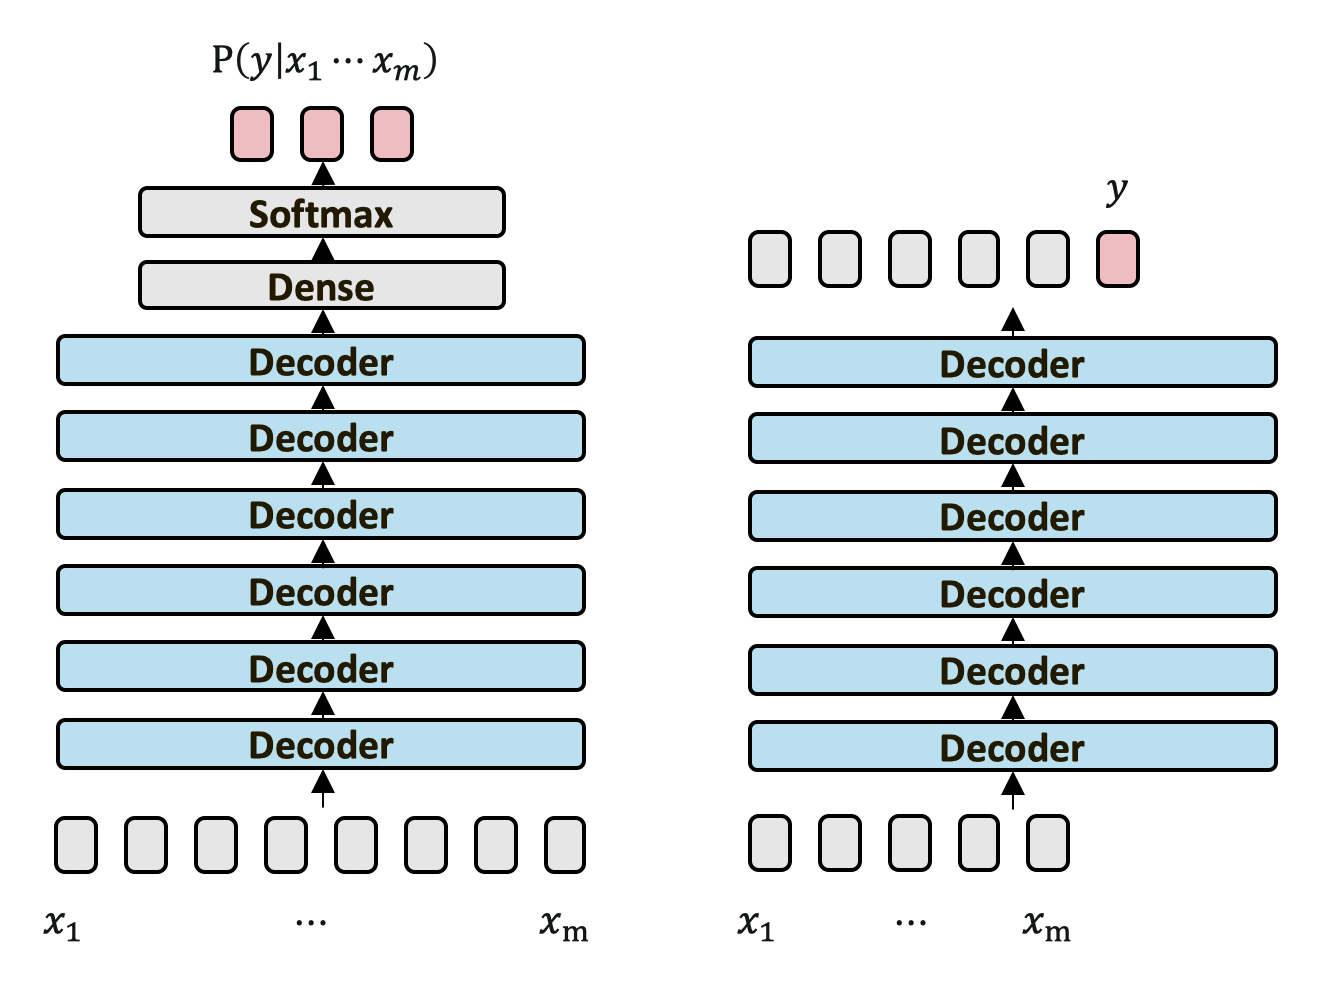
\includegraphics[width=10cm]{images/generative-2.png}
\end{center}
\caption{Configurations for auto-regressive language models at inference. (left) standard configuration with dense and softmax layers (right) generative configuration for which the target is directly predicted as a sequence of words in natural language.}
\labfig{generative:inference}
\end{figure}

\paragraph{Few or zero-shot(s) learning} \acomment{Pushing the paradigm to its limit, it is possible to solve tasks using a generative formalism without updating the model weights. Such procedures are referred to as few or zero-shot(s) learning. These configurations also use the generative task format. However, we will add information to the input natural language sequence: the \textit{prompt} contains directions for the model to solve the task. Typically the prompt contains a brief description of the task (zero-shot), supplemented by one or few examples and their corresponding labels (one and few-shot(s)). A typical language prompt will contain the concatenation of $k$ examples and their corresponding labels $x^k_1 \cdots x^k_m [SEP] y^k$, followed by the example to predict $x_1 \cdots x_m$ without its label (\refeq{generative:few-shot} and \refeq{generative:few-shot-proba-m+1}).

\begin{align}
    h^N &= \textrm{GPT}(\textrm{task description} \nonumber \\
    & \quad x^1_1 \cdots x^1_m [SEP] y^1 \nonumber \\
    & \quad x^2_1 \cdots x^2_m [SEP] y^2 \nonumber \\
    & \quad x_1 \cdots x_m [SEP]) \labeq{generative:few-shot}\\
    \hat{y} &= \textrm{softmax}(h^N W_e^T) \labeq{generative:few-shot-proba-m+1}
\end{align}

For example, if we aim at solving a question answering task, we can format the following prompt to answer the question "Que célèbre-t-on le 14 juillet ?": 

Q : Qui est Superdupont ?\\
R : Superdupont un super-héros français, patriote et chauvin.\\
\#\#\#\\
Q : Qui était le président de la France en 1982 ?\\
R : Francois Mitterrand.\\
\#\#\#\\
Q : Qu'est-ce qu'un algorithme ?\\
R : Un algorithme est une suite finie et non ambiguë d'instructions et d’opérations permettant de résoudre une classe de problèmes.\\
\#\#\#\\
Q : Que célèbre-t-on le 14 juillet ?
R :

In this configuration, we do not fine-tune the model on the task. We only use the prompt to control the input fed to the model. The success of this approach seems closely related to the model size \parencite{brown_20}.}

% Pre-trained auto-regressive models leverage the generative properties of language models by employing an \bcomment{alternative}{what do you mean by alternative} training and inference paradigm \parencite{radford_2018, radford_2019, brown_20}. \bcomment{With this paradigm, the model directly generates the answer in natural language}{the paradigm should be detailed earlier}, allowing them to accomplish a variety of tasks without changing the architecture. \bcomment{Fhurthermore, this setup doesn’t require to fine-tune the model weights on examples specific to the task}{which setup ? you should define the model first and explain that as it is auto-regressive it can be used to generate text from prefixes}. 
% Still, the generality of what are sometimes called \bcomment{"foundational"}{cite} models \parencite{bommasani_21} has some limitations.  We use the same architecture as the OpenAI GPT in English. \sidenote{We used the implementation from the open-source library Transformers: \url{https://huggingface.co/}.}. 
% \bcomment{add a paragraph stating that you can either use the model in a fine-tuning scenario or as an auto-regressive generator without fine tuning}{}

% Une fois le modèle pré-entraîné, il est possible de l’utiliser suivant deux types de scénarios. On peut ajouter une couche spécifique à la tache en sortie du modèle et ajuster l’ensemble des paramètres comme on le ferait pour d’autres modèles pré-entraînés comme Bert. On décrit la tâche comme un jeu de données $C$ ou chaque instance consiste en une séquence de tokens $x^1 \cdots x^m$ et un label $y$. Les données sont transformées par le modèle. On considère $h_l^m$, la représentation du dernier token d’un exemple donné par la dernière couche de transformers. 

% Pour prédire $y$, on passe cette représentation dans une couche dense avec des paramètres $W_y$ suivie par un softmax : $P\left(y \middle| x^1 \cdots x^m \right)=softmax(h_l^m W_y)$. On cherche alors à maximiser la fonction de coût : $L(C)=logP\left(y \middle| x^1 \cdots x^m\right)$.

% \textbf{Reformulation de la tâche pour tirer parti du modèle génératif} : La méthode par ajustement suppose néanmoins de modifier l’architecture du modèle en ajoutant une couche spécifique à la tâche. Il est également possible de formaliser les tâches pour tirer parti des propriétés génératives du modèle. Suivant ce scénario, on transforme le jeu de données. Une instance est une séquence de tokens à laquelle on ajoute un token de séparation, et le label à prédire $y$ de telle sorte que l'instance prenne la forme $x^1,\cdots,x^m,SEP,y$. 
% Lors de la prédiction, l'instance à prédire prend alors la forme $x^1,\cdots,x^m,SEP$. On interprète la probabilité de générer le token associé à une classe comme la probabilité de la classe. Cette formulation se généralise au cas où la classe $y$ est plus complexe qu’un simple label. Dans le cas de traduction automatique ou de résumé automatique, $y$ correspond à la séquence de tokens du texte de référence.

\section{Pre-training corpora}
\labsec{generative:corpus}

For pre-training, generative transformers require only raw text. However, training such models requires large corpora due to their large number of parameters. \acomment{We need not only a large corpus but also one with good properties. Specifically, we expect the document length to be relatively close to the size of the context. We plan on organizing the training by collecting documents in batches, which means padding all documents to the same length—in our case, the context size. A document that is significantly shorter than the context size will require a lot of padding that will not contribute to the final calculation of the loss. Consequently, such computations will be "lost", a side-effect we want to avoid. GPT context size is typically longer than \bert. Consequently, \gpt training requires longer documents than \bert.} The majority of the corpora used to adapt \textsc{Bert} in French: Camembert \parencite{martin_20} or Flaubert \parencite{le_20b, le_20a} use relatively short documents. \acomment{Since the sequential order of the documents was not preserved, we couldn't re-aggregate them directly and build our own corpus.} We instead aggregated two other training corpora with different scales to train our models. We summarize their main statistics in \reftab{generative:corpus-size}.

\begin{table*}[!htb]
\footnotesize
\centering {
\begin{tabularx}{16cm}{@{}l | Y Y Y Y@{}}
\toprule
\textbf{Models} & \textbf{OpenAI GPT} &  \textbf{OpenAI GPT-2} & \textbf{$\text{GPT}_{fr}$-124M} & \textbf{$\text{GPT}_{fr}$-1B} \\
\midrule
\midrule
% Modèles & Nombre de documents ($\times 10^6$) & Nombre de mots ($\times 10^9$)
% OpenAI GPT & 2,262,211$^\dagger$ & 1,158,252,402$^\dagger$   \\
% OpenAI GPT-2 & 8,000,000 & 4,680,000,000$^\dagger$ \\
% Fr GPT-124M & 1,656,080 & 1,597,377,426 \\
% Fr GPT-1B & 7,356,862 & 3,106,521,195
\# Documents ($\times 10^6$) & 2.3$^\dagger$ & 8.0 & 1.7 & 7.4 \\
\# Tokens ($\times 10^9$)& 1.2$^\dagger$ & 4.7$^\dagger$ & 1.60 & 3.1\\
Avg. tokens per document & \numprint{512}$^\dagger$ & \numprint{585}$^\dagger$ & \numprint{965} & \numprint{422}\\
\bottomrule
\end{tabularx}}
\caption{\labtab{generative:corpus-size} Statistics of the corpora used to pre-train the models. The $\dagger$ denote estimates based on the available data. Specifically, we hypothesize that the number of tokens per document is equal to the context size for OpenAI GPT. We estimate the OpenAI GPT-2 statistics using the open-source sample: \url{https://github.com/openai/gpt-2-output-dataset}.}
\end{table*}

We create a first corpus, used to train the first model $\text{GPT}_{fr}$-124M, as an aggregation of existing corpora: Wikipedia\sidenote{\url{https://dumps.wikimedia.org/frwiki/}}, OpenSubtitle\sidenote{\url{http://opus.nlpl.eu/download.php?f=OpenSubtitles/v2016/mono/}} \parencite{tiedemann_12} and Gutenberg\sidenote{\url{http://www.gutenberg.org}}. We divide documents into successive sentences and concatenate them into documents of maximum \numprint{1024} tokens\sidenote{\acomment{We use this sentence-level division to build our documents to avoid pitfalls such as creating documents starting or ending with only part of a sentence or mixing two very distinct original documents into one.}}.

We then create a second corpus to train our model with above 1 billion parameters: $\text{GPT}_{fr}$-1B. Our approach is to augment the first corpus with data from the Common Crawl\sidenote{\url{http://data.statmt.org/ngrams/deduped2017/}} in French. \acomment{The Common Crawl data typically contains many poorly formatted, inconsistent documents. We therefore apply strong filters to select a portion of the Common Crawl, whose distribution is close to our first corpus. We take inspiration from the procedure outlined in \textcite{brown_20}, and filter the Common Crawl data in several steps.}
\begin{itemize}
    \item First, we exclude all the documents too short with less than 128 tokens, as done in \textcite{shoeybi_19}. We filtered out 93\% of the raw documents using this very simple filter; 
    \item We then filter out documents whose word distribution differed too much from the first corpus. By using \numprint{200000} randomly chosen documents, we train a binary classifier to discriminate between documents in the first corpus and those in the Common Crawl. We excluded all documents that had a probability <10\% to be extracted from the first corpus. The filter, deliberately unselective, is designed to filter out explicitly invalid or poorly formatted documents;
    \item Finally we apply a filter targeting the structure of documents. We selected documents with a low perplexity\sidenote{Given a sequence $U=\{u_1 \cdots u_T\}$, we define the perplexity as: $PPL(U) = exp \left(-\frac{1}{T}\sum_{t=1}^{T}\log p_{\theta}(u_t|u_{<t})\right)$ with $\log p_{\theta}(u_t|u_{<t})$ the conditional log-likelihood given our model for the $t$th token given the previous tokens $u_{<t}$.} according to the model $\text{GPT}_{fr}$-124M. To preserve documents out of the distribution, we fixed a threshold $g$. With $g$ the realisation from a Pareto law $G \sim \mathcal{G}(\alpha)$. We keep the document if its perplexity $ppl$ verifies: $g > ppl / ppl_{th}$. With the threshold $ppl_{th}$ set to $60$. \sidenote{\acomment{This selection using a pareto distribution is directly inspired from the procedure used in \textcite{brown_20}. The threshold of 60 is calibrated empirically so that, upon application of the filter, the expected number of documents are returned.}}
\end{itemize}
% \bcomment{explain further at the beginning of the section what goal you try to achieve when applying these filters}{error in footnote 7 sequence up to $u_T$}

% By tokens, we refers to \bcomment{Lastly, the model use a bytepair vocabulary encoding (BPE) with \numprint{50000} units \parencite{sennrich_16a} trained on the first corpus used for the pre-training of $\text{GPT}_{fr}$-124M.}{comes too late, why training BPE only on this corpus ?}
% Parler ici de l'entrainement du vocabulaire

\section{Pre-training}
\labsec{generative:training}

% L’attention est suivie de couches denses. 
%Le modèle peut finalement être décrit simplement selon les équations suivantes :

% \begin{equation}
%     \mathcal{L}(U)= \sum_i log P\left(u_{i} \middle| u_{i-k} \cdpts u_{i-1}  ; \Theta\right)
% \end{equation}


% \begin{gather}
% \begin{align}
%     h_0 &= UW_e+W_p \\
%     h_i &= \textrm{transformeur\_decodeur}(h_{i-1}), \quad \forall i \in [1,n] \\
%     P\left(u \middle| U \right) &= softmax(h_n W_e^T )
% \end{align}
% \end{gather}

% Avec $U=\{u_{-k} \cdots u_{-1}\}$ le vecteur d’embeddings des tokens du contexte, $n$ le nombres de couches, $W_e$ la matrice d’embeddings et $W_p$ la matrice d’embeddings positionnels.

% \paragraph{Paramètres pour l'entraînement des modèles}
% \label{sec:models}

\subsection{Architectures} 

We pre-trained two models, one of which had over 1 billion parameters, as detailed in \reftab{generative:model-def}. Based on the work from \textcite{shoeybi_19}, which compares many training configuration, we proposed an architectures avoiding the use of model parallelization. Indeed, spreading model modules across multiple compute units is a major factor slowing down training.

\begin{table*}[!ht]
\footnotesize
\centering {
\begin{tabularx}{16cm}{@{}l|YYYYY@{}}
\toprule
% Modèle & Taille du contexte & Nombre de couches & Nombre de têtes d'attention & Dimension du modèle  & Nombre de paramètres\\\hline
% Fr GPT-124M & 1024 & 12 & 12 & 768 & 124,242,432 \\	
% Fr GPT-1B & 1024 & 24 & 14 & 1792 & 1,016,841,728\\
% OpenAI GPT & 512 & 12 & 12 & 768 & \hl{124,242,432} \\
% OpenAI GPT-2 & 1024 & 48 & 25 & 1600 & \hl{1,558,000,000} \\
\textbf{Models} & \textbf{OpenAI GPT} &  \textbf{OpenAI GPT-2} & \textbf{$\text{GPT}_{fr}$-124M} & \textbf{$\text{GPT}_{fr}$-1B} \\
\midrule
\midrule
Context size & 512 & \numprint{1024} & \numprint{1024} & \numprint{1024} \\
\# Layers & 12 & 48 & 12 & 24 \\
\# Attention heads & 12 & 25 & 12 & 14 \\
Embeddings size & 768 & \numprint{1600} & 768 & \numprint{1792} \\
\# Parameters ($\times 10^6$) & 117 & \numprint{1558} & 124 & \numprint{1017}\\
\bottomrule
\end{tabularx}}
\caption{\labtab{generative:model-def} Statistics of the architectures and comparison with OpenAI models \parencite{radford_2018, radford_2019}.}
\end{table*}

\subsection{Infrastructures}

We pre-train the $\text{GPT}_{fr}$-124M models on a TPU v2-8 using the Google Colab interface\sidenote{\url{https://colab.research.google.com}}. We train the $\text{GPT}_{fr}$-1B on the French super-computer Jean Zay\sidenote{\url{http://www.idris.fr/jean-zay/}}. We perform a total of 140 hours of computation on Tesla V100 hardware (300W TDP). We distribute the training on 4 compute nodes of 8 GPUs. We used data parallelization in order to divide each micro-batch on the computational units. We estimated the total emissions at 580.61 kgCO$_2$eq\sidenote{We estimated the equivalent emissions using the Machine Learning Impact calculator (\url{https://mlco2.github.io/impact}) introduced in \textcite{lacoste_2019}.}.

\subsection{Hyper-parameters}

% dire que ce modèle est un des premiers à avoir été entrainé sur l'IDRIS, mettre en avant dans le chapitre le coté infrastructure : calcul distribué, combien de noeuds, temps d'entrainement etc.
We share the same set of hyper-parameters for the two models. We set the learning rate to $1.5e^{-4}$ with a \numprint{2000} warm-up steps followed by a cosine decay. We pre-trained the models for \numprint{125000} iterations using a batch size of 128 documents and half-precision \parencite{micikevicius_18}. We kept \numprint{6080} documents to constitute a validation set. We can follow the evolution of the perplexity on this validation set in \reffig{generative:ppl-training}. The other parameters (initialization, dropout ...) are set according to \textcite{radford_2018}.

\begin{figure*}[!htb]
\begin{center}
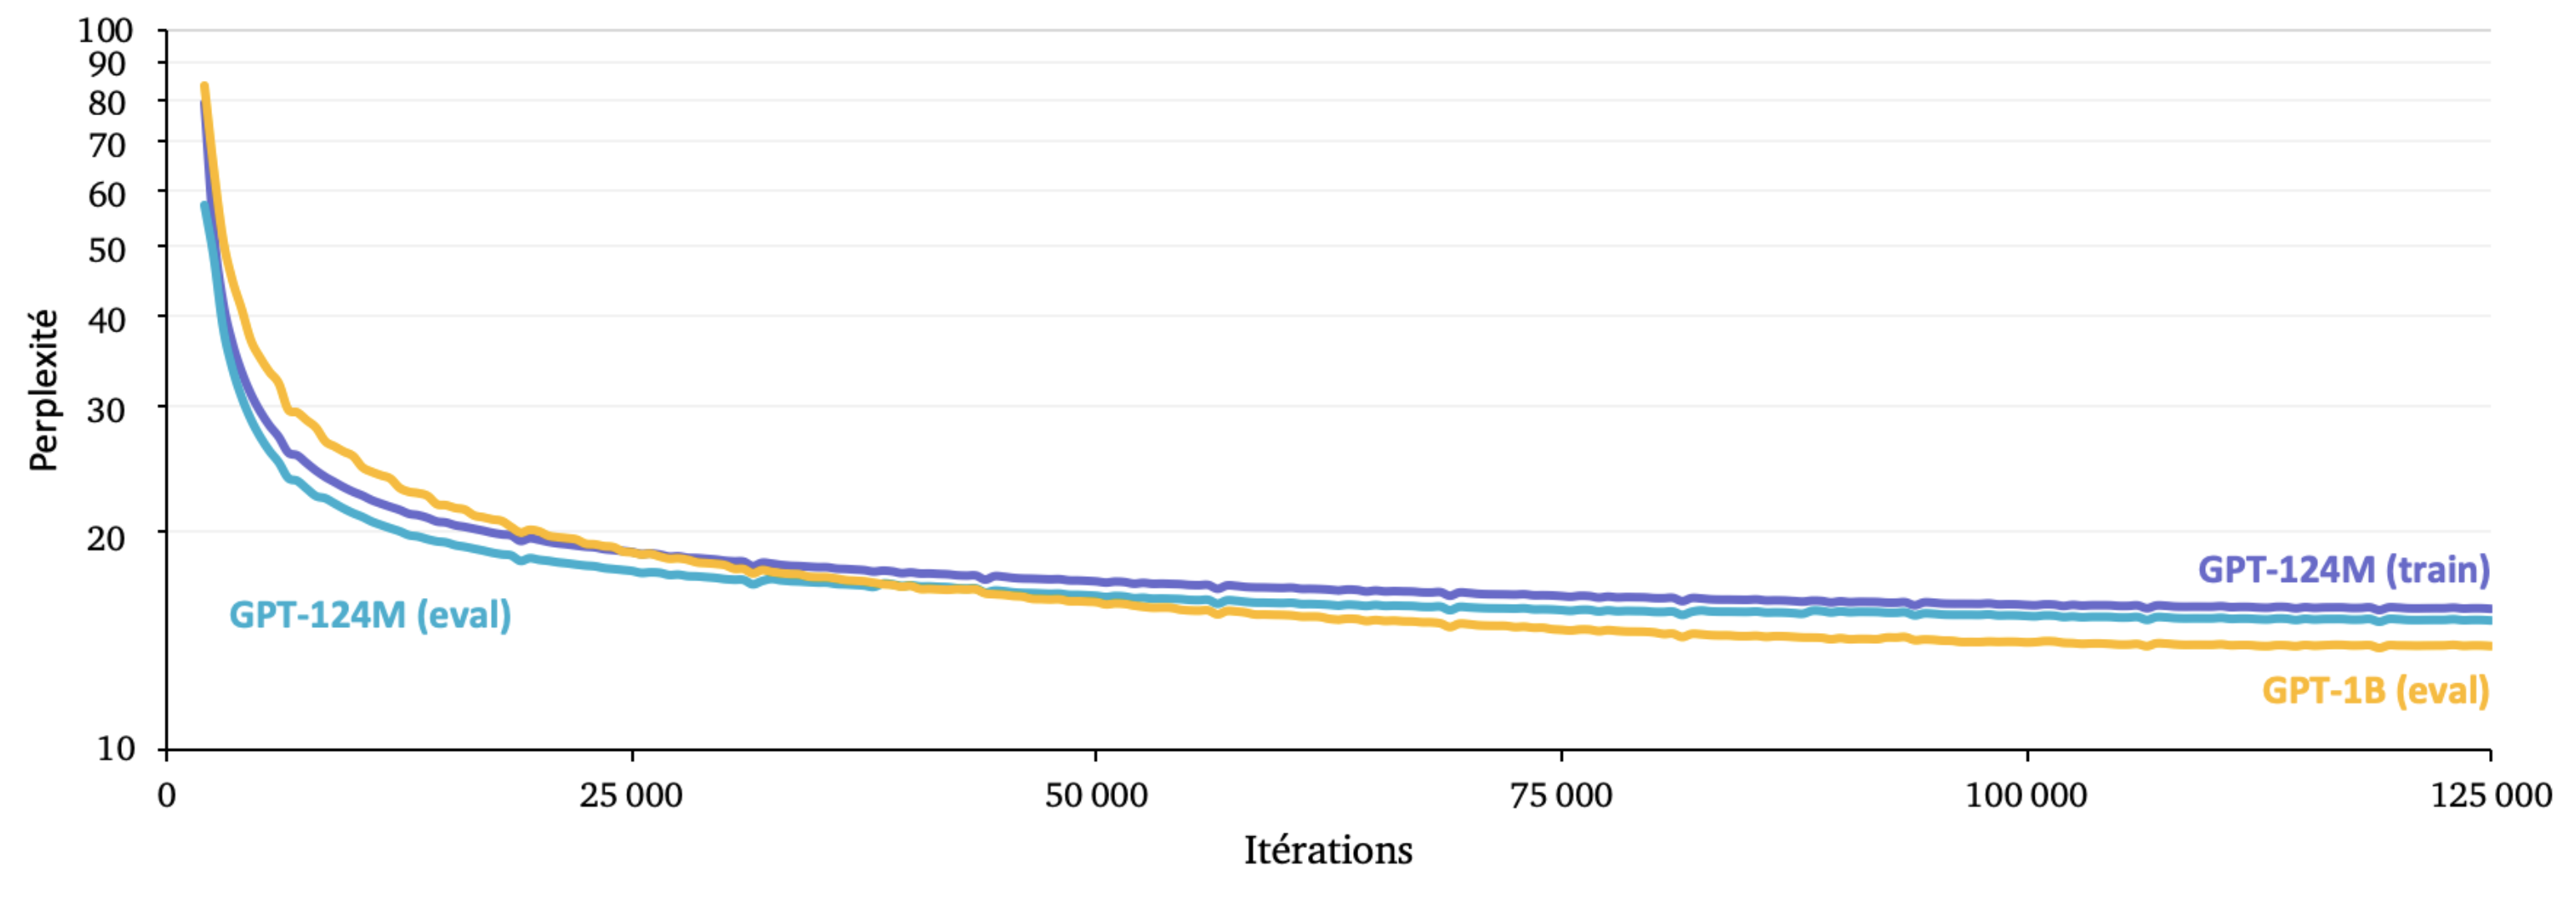
\includegraphics[width=16cm]{images/ppl-training-5.png}
\end{center}
\caption{Evolution of perplexity during model training. The evaluation set is the same for both models.}
\labfig{generative:ppl-training}
\end{figure*}

\section{Evaluation}
\labsec{generative:evaluation}

\subsection{Language generation}

\acomment{Language models are very effective for consistent natural language generation.} Even though the pre-training objective is relatively simple, deep neural networks may acquire shocking grammar abilities \parencite{linzen_2020}. For example, the English GPT-2 generates correct text with plural and long-distance agreement despite any prior linguistic knowledge. Such agreements are determined by abstract structures and not just linear order of words. Surprisingly, models can learn such specific linguistic patterns (subject-verb, noun-adverb, verb-verb) with no prior information about linguistic theory. 

\acomment{We give an example of text generation below. We give the first sentence from \'{A} la recherche du temps perdu as input to our model $\text{GPT}_{fr}$-1B, which generates the following sentences as output. As observed in \textcite{linzen_2020}, the text is consistent with the input prompt, without orthographic or grammar mistakes. We observe even \bcomment{complex}{unusual} verb forms such as "habillasse". Nonetheless, we observe some inconsistencies, such as "un homme entra, vêtu d'un long manteau d'homme" which seems repetitive. Moreover, while the model can generate text with up to \numprint{1024} tokens, generated text lack a narrative structure one would typically expect from a human-generated story.

\texttt{\textbf{Longtemps je me suis couché de bonne heure.} La nuit se faisait assez obscure, les étoiles semblaient dormir de temps à autre, cependant le peu de clarté qui me permit de marcher la nuit dans la chambre éveilla en moi une profonde pitié de ce que je faisais là, et cette peur de l'avenir me devint plus vive et plus aiguë. Je me réveillai en sursaut, comme un homme ivre qui s'endort en repassant sa bière. Je passai rapidement le seuil de la porte, et un homme entra, vêtu d'un long manteau d'homme et portant un paquet à la main. Je lui demandai la permission d'entrer. Il me répondit qu'il viendrait demain, et qu'il ne pouvait pas attendre, à cause des travaux de la nuit. Il était habillé simplement, et l'homme me dit qu'il ne voulait pas me donner d'argent; seulement, il voulait que je m'habillasse, pour aller dans le même train \textup{[\,\dots]}}}

\paragraph{WikiText-FR}\acomment{To better quantify our model's abilities to produce consistent text, we created WikiText-FR. This benchmark evaluates French language model generation abilities by measuring their perplexity on reference texts. Perplexity is a metric for evaluating language models. It does not measure the model's performance on a specific task like translation or automatic summarization but gives an intrinsic measure of its ability to generate text. It can thus be used to compare models between them\sidenote{The perplexity $PP$ is defined for a sequence of words $W = w_1 \cdots w_N$ as $PP(W) = P(W)^{-1/N}$ with $N$ the length of the sequence and $P(W)$ the probability assigned by the model to the sentence. Thus, the higher the probability $P(W)$ assigned by the model to the sentence $W$, the lower the perplexity $PP(W)$.}.

We want our model to assign a high probability to correct sentences (without grammatical error, in French, without spelling mistakes...). On the contrary, we want it to attribute a low probability to incorrect sentences (and thus a high perplexity in this case). To do this, we evaluate the perplexity of the model on a test set that we know is correct. In the same vein as the English work, we developed two corpora based on Wikipedia to evaluate French language models. We collected the text from article labeled as “featured articles”\sidenote{\url{https://en.wikipedia.org/wiki/Wikipedia:Featured_articles}} or “good articles”\sidenote{\url{https://en.wikipedia.org/wiki/Wikipedia:Good_articles}}. Such articles have been manually reviewed and distinguished for their quality. Models are then evaluated by measuring the perplexity on this test set. A low perplexity indicates that the probability distribution produced by the model is good at predicting the sample.}

%presented in \refsec{generative:corpus}. 

% \paragraph{Language model evaluation corpus} 
%\bcomment{maybe explain a little bit why wikipedia only ? and not e.g. extracting a small sample from the train set}{}
Since pre-processing Wikipedia articles is not straightforward, we extracted the raw text directly from the Wikipedia API. We gathered \numprint{2246} good articles and \numprint{3776} featured articles, over the period of 2003 to 2020. We did not apply any specific pre-processing. Transformer models indeed use a dedicated tokenization with very few out-of-vocabulary tokens. The corpora statistics are presented in \reftab{generative:wikitext} and are available as open-source contributions\sidenote{\url{https://huggingface.co/datasets/asi/wikitext_fr}}. We emphasize that \textbf{we specifically filtered these articles out of the pre-training corpora.}

%\bcomment{???}{we miss a transition from the prev parag} 
The \textbf{WikiText-2-FR} consists in a random train/valid/test split of the featured articles with respectively \numprint{2126}/60/60 articles. The \textbf{WikiText-72-FR} share the same valid and test set. However the training set includes the concatenation of \textbf{WikiText-35-FR} training set and all good articles.

\begin{table*}[!ht]
\footnotesize
\centering {
\begin{tabularx}{16cm}{@{}l| Y Y c c | Y Y c c@{}}
\toprule
& \multicolumn{4}{c}{\textbf{WikiText-EN}} & \multicolumn{4}{c}{\textbf{WikiText-FR}} \\
& Valid & Test & Train-2 & Train-103 & Valid & Test & Train-35 & Train-72 \\
\midrule
\midrule
Documents & 60 & 60 & 600 & \numprint{28475} & 60 & 60 & \numprint{2126} & \numprint{5902}\\
% 217,646 & 245,569 & 2,088,628 & 217,646 & 245,569 & 103,227,021 & 896,385 & 896,818 & 35,166,441 & 896,385 & 896,818 & 72,961,483
Tokens ($\times 10^3$) & 218 & 246 & \numprint{2089} & \numprint{103227} & 896 & 897 & \numprint{35166} & \numprint{72961}\\
Vocabulary & & & \numprint{33278} & \numprint{267735} & & & \numprint{137589} & \numprint{205403}\\
Out of Vocabulary (\%) & & & 2.6 & 0.4 & & & 0.8 & 1.2 \\
\bottomrule
\end{tabularx}}
\caption{\labtab{generative:wikitext}Descriptive statistics for the corpora \textbf{WikiText-FR}. We evaluate the vocabulary size using the MOSES tokenizer \parencite{koehn_07}. Tokens out of vocabulary correspond to those that occur less than three times.}
% et remplacés par la marque <unk> pour l'ensemble du corpus.}
\end{table*}

Since the pre-training and evaluation corpora are close, we do not fine-tune the model. We directly present the perplexity measured on the test set in \reftab{generative:lm-scores}. We precise that we evaluate the perplexity based on the tokenization inherent to the model. The latter is the same for $\text{GPT}_{fr}$-124M et 1B but may be different for other models. In particular, we considered language models with 5-grams and kneser-ney smoothing \parencite{ney_94} using the SRILM tool \parencite{stolcke_02} as baseline.

%TODO relire précisemment à partir d'ici
The approaches are not directly comparable because the tokenization is different and our model is trained on a much larger volume of data. The results in \reftab{generative:lm-scores} are therefore given for illustrative purposes but highlight the performance of our $\text{GPT}_{fr}$-1B model. 
%\bcomment{the table is unclear}{}

\begin{table*}[!ht]
\footnotesize
\centering {
\begin{tabularx}{16cm}{@{}l | Y Y Y @{}}
\toprule
% Modèle & WikiText-35-FR & WikiText-72-FR \\\hline
% $\text{GPT}_{fr}$-124M & \hl{15} & \hl{16} \\	
% $\text{GPT}_{fr}$-1B & \hl{14} & \hl{14}
\bcomment{\textbf{Models}}{remove this label} & \textbf{5-grams} & \textbf{$\text{GPT}_{fr}$-124M} & \textbf{$\text{GPT}_{fr}$-1B} \\
\midrule
\midrule
WikiText-35-FR (ppl) & 166.7 & 109.2 & \acomment{\textbf{12.9}} \\
WikiText-72-FR (ppl) & 99.1 & 109.2 & \acomment{\textbf{12.9}} \\
\bottomrule
\end{tabularx}}
\caption{\labtab{generative:lm-scores}Perplexity of our models. We did not update the models on the training set and the perplexity is directly measured on the test set which are identical for two benchmarks. The n-gram model is trained on the corresponding training corpora.}
\end{table*}

% \bcomment{Prédiction zeo shot et résumé automatique pour dire que on va s'intéresser à cette propriété et rappel section 2.2 C'est l'inétert du mdoèle. Commentaire avec ce qu'on donne comme input. et formattage de la tache. Dire que le modèle n'est pas entraîné. Dire que forme de requête et setup très différent de d'habitude.}

\subsection{Automatic summary} 

We then evaluate our models on an automatic summary task, which exploits the generative properties of the model. We use the configuration proposed in \cite{radford_2018} which allows to use the model without adjusting its architecture. We simply add the pattern \acomment{\textit{"Pour résumer :"}} after the original text to encourage the model to generate text that summarizes posts. For OpenAI GPT-2, the added pattern is "TL;DR:" which stands for "Too Long; Didn't Read." and is used on the Reddit forum\sidenote{\url{https://www.reddit.com/}} as a marker to summarize a discussion. \acomment{It should be noted that "TL;DR:" does not have a real equivalent in French. Most likely, this pattern is present in the English pre-training data for GPT-2, while it is absent from the French data used for the pre-training of $\text{GPT}_{fr}$. In a sense, \cite{radford_2018} take advantage of a regularity in the pre-training data to benefit from a specific behavior during inference.}
% \bcomment{you should discuss these choices in more details comparing the situation on French and English}{}

\begin{table*}[!htb]
\footnotesize
\centering {
\begin{tabularx}{16cm}{@{}X@{}}
\toprule
\textbf{Extract of the input article}: Présenté comme l'origine des explosions dévastatrices à Beyrouth qui ont fait plus d'une centaine de morts et au moins 4.000 blessés, le nitrate d'ammonium est principalement employé comme engrais azoté, mais peut aussi entrer dans la composition de certains explosifs à usage civil. \textup{[\,\dots]} L'association "Sauvons la baie de saint-Brieuc" a été créée en début d'année pour alerter la population sur ce danger et mettre fin au transport de nitrate d'ammonium.\\
\textbf{Reference}: Ces cargaisons dangereuses font l'objet de mesures de sécurité très strictes et il n'y a jamais plus de 7.500 tonnes de nitrate d'ammonium dans le port en même temps.\\
\textbf{Generated summary}: les nitrates sont dangereux pour la santé et la sécurité des personnes et des biens.\\
\midrule
\textbf{Extract of the input article}: Au micro de RTL dimanche matin, la candidate à la mairie de Paris Rachida Dati n'a pas tardé à décrypter un récent sondage qui la donne en progression pour les prochaines municipales à Paris face à Anne Hidalgo. \textup{[\,\dots]} Appelée "Paris d'Avenirs", elle consisterait en une aide de 1.200 euros par an pendant trois ans, à l'arrivée d'un nouvel enfant. Mme Dati prévoit un coût de 20 millions d'euros par an pour cette mesure.\\
\textbf{Reference}: Invitée sur RTL ce dimanche, la candidate à la mairie de Paris a expliqué que "les Parisiens attendent une solution au déclin de Paris".\\
\textbf{Generated summary}: le maire de la capitale est "un homme de gauche" et "une femme de droite".  PRÉSIDENTIELLE >> Inscrivez-vous pour recevoir en temps réel les résultats de votre ville partages les opinions, résultats par ville, profession, catégorie socioprofessionnelle, etc.\\
\bottomrule
\end{tabularx}
\caption{\labtab{generative:summary-examples} \acomment{Examples extracted from the OrangeSum tasks and summaries automatically generated with $\text{GPT}_{fr}$.}}
\end{table*}

We considered the OrangeSum dataset for the abstract summary \parencite{kamal_20}. \acomment{We give some text, summary pairs from the task in \reftab{generative:summary-examples}.}
% \bcomment{Examples would be welcome}{}
We complete the text using the top-k random sampling strategy \parencite{lewis_18} with $k=2$\sidenote{\acomment{In top-K sampling, we generate words sequentially. At each time step, we retain the K most likely next words and normalize their probabilities. We sample the next word based on this probability distribution. The process is therefore non-deterministic.}}. We keep the first 3 sentences from the first 100 generated tokens. \acomment{Using ROUGE metrics\sidenote{The ROUGE metrics are a collection of metrics that allows comparing automatic summaries with a reference text by calculating the proportion of "n-grams" that are common between the two texts.} \parencite{lin2004rouge}, we compare our model to the reference, which considers the first sentence of the text as a summary. \reftab{generative:sum} shows that, in this complex configuration, our models just manage to approach the proposed reference.}

\begin{table*}[!ht]
\footnotesize
\centering {
\begin{tabularx}{16cm}{@{}l | Y Y Y | Y Y Y@{}}
\toprule
& \multicolumn{3}{c}{\textbf{Synthesis}} & \multicolumn{3}{c}{\textbf{Title}} \\
& R1 & R2 & RL & R1 & R2 & RL \\
\midrule\midrule
First sentence & \textbf{22.1} & \textbf{7.1} & \textbf{15.3} & \textbf{18.6} & \textbf{7.7} & \textbf{15.0} \\
% 3 phrases aléatoires & 24,2 & 6,9 & 15,0 & 12,6 & 4,0 & 9,5 \\\hline
$\text{GPT}_{fr}$-124M & 17.5 & 3.1 & 12.1 & 13.9 & 2.3 & 9.7 \\
% $\text{GPT}_{fr}$-124M (Fine tuned) & 21,0 & 2,7 & 12,8 & --- & --- & --- \\
$\text{GPT}_{fr}$-1B & 16.6 & 3.4 & 11.5 & 10.2 & 2.6 & 8.4 \\
\bottomrule
\end{tabularx}}
\caption{Comparison of the generated abstracts with the title of the article or the proposed synthesis. We use the ROUGE score and the OrangeSum corpus \parencite{kamal_20}. Our models are used in learning without examples and thus without updating the parameters on the training set. We indicate the best results in \textbf{bold}.}
\labtab{generative:sum}
\end{table*}

We have manually analyzed examples. The generated text is correct in terms of spelling and syntax. It is also in line with the theme and in continuity of the proposed articles. Nevertheless, the generated text generally focuses on a specific detail of the article and then expands on it by sometimes inventing elements. This phenomenon is known as \textit{hallucination} \parencite{kryscinski_19}. \acomment{As illustrated in \reftab{generative:summary-examples}}, the method allows to generate coherent text but does not manage to synthesize completely the general idea of the text.
% \bcomment{examples would be welcome}{}

\subsection{FLUE benchmark} 

Generative models extend some of the perspectives of \textsc{Bert} type models. Nevertheless, this type of pre-training does not allow to reach the same performances as models taking into account the whole context. When we directly compare the English models on the GLUE benchmark, we observe an average difference of more than 4 points between OpenAI GPT and \textsc{Bert}-base \parencite{radford_2018}. We still compared our model on the French FLUE benchmark in \reftab{generative:flue}.

\begin{table*}[!htb]
\footnotesize
\centering {
\begin{tabularx}{16cm}{@{}X X c@{}}
\toprule
\multicolumn{2}{c}{\textbf{Examples}} & \textbf{Labels}\\
\midrule
\multicolumn{3}{c}{\textbf{CLS}}\\
\midrule
% \multicolumn{2}{@{}X@{}}{}
un conte moderne des temps anciens ; une poésie dans les images ; dépaysement et humour garanti ... & --- & Positif \\
N'apporte strictemant rien de plus de ce qui est connu. SANS INTERET. & --- & Négatif \\
\midrule
\multicolumn{3}{c}{\textbf{XNLI}}\\
\midrule
Mon Walkman S' est cassé alors je suis en colère maintenant je dois juste tourner la stéréo très fort & Je suis contrarié que mon walkman soit cassé et maintenant je dois tourner la stéréo très fort . & Entailment\\
Qu' est-ce que tu en sais ? Tout ceci est à nouveau leur information . & Cette information leur appartient . & Entailment\\
L' homme aurait dû mourir sur le coup . & L' homme allait parfaitement bien . & Contradiction\\
Et C' est sympa de vous parler tous les deux~. & Je te parle tous les jours . & Neutral\\
\midrule
\multicolumn{3}{c}{\textbf{PAWS-X}}\\
\midrule
C'est le siège du district de Zerendi dans la région d'Akmola. & C'est le siège du district de Zerendi dans la région d'Akmola. & Positif\\
Elizabeth II était un ancêtre des reines Edzard II et Beatrix des Pays-Bas. & Edzard II était un ancêtre des reines Elizabeth II et de la Béatrix des Pays-Bas. & Négatif\\
Saunders a battu Dan Barrera à l'unanimité. & Par décision unanime, Dan Barrera a battu Saunders. & Négatif\\
\bottomrule
\end{tabularx}
\caption{\labtab{generative:flue-examples} \acomment{Examples extracted from the CLS, XNLI and PAWS-X tasks.}}
\end{table*}

We considered the following tasks, \acomment{for which we present example samples in \reftab{generative:flue-examples}}:
%\bcomment{More details and examples on the tasks would be welcome}{}
\begin{itemize}
    \item CLS is a dataset composed of reviews on Amazon to be classified as positive or negative. It contains 3 product categories: books, DVDs and music. Each category is divided in \numprint{2000} examples of training, validation and evaluation. 
    \item PAWS-X contains pairs of sentences. It is a binary classification task to identify pairs whose two sentences are semantically equivalent. There are \numprint{49401} examples for training, \numprint{1992} for validation and \numprint{1985} for evaluation.
    \item XNLI contains pairs of sentences. The task is to predict whether the first (premise) implies the second (hypothesis). \numprint{392702} pairs are used for training, \numprint{2490} pairs for validation and \numprint{5010} pairs for evaluation.
\end{itemize}

This time the weights of our model are updated. The hyper-parameters are set according to the recommendations of \textcite{le_20b, le_20a}. As expected, the performance of the model does not reach those obtained with models of type \textsc{Bert}. 

\begin{table*}[!ht]
\footnotesize
\centering {
\begin{tabularx}{16cm}{@{}l | Y Y Y Y Y Y@{}}
\toprule
\multirow{2}{*}{\textbf{Models}} & \multicolumn{3}{c}{\textbf{CLS}} & \multirow{2}{*}{\textbf{PAWS-X}} & \multirow{2}{*}{\textbf{XNLI}} & \multirow{2}{*}{\textbf{Avg.}} \\
 & Books & DVDs & Music & & & \\
\midrule
\midrule 
mBERT$^\dagger$ \parencite{devlin_19} & 86.2 & 86.9 & 86.7 & 89.3 & 76.9 & 85.2 \\
CamemBERT$^\dagger$ \parencite{martin_20} & 92.3 & 93.0 & 94.9 & \textbf{\underline{90.1}} & 81.2 & 90.3 \\
FlauBERT-base$^\dagger$ \parencite{le_20a, le_20b} & 93.1 & 92.5 & 94.1 & 89.5 & 80.6 & 90.0 \\
FlauBERT-large$^\dagger$ \parencite{le_20a, le_20b} & \textbf{\underline{95.0}} & \textbf{\underline{94.1}} & \textbf{\underline{95.9}} & 89.3 & \textbf{\underline{83.4}} & \textbf{\underline{91.5}} \\\midrule
$\text{GPT}_{fr}$-124M & 88.3 & 86.9 & 89.3 & 83.3 & 75.6 & 84.7 \\
$\text{GPT}_{fr}$-1B & \textbf{91.6} & \textbf{91.4} & \textbf{92.6} & \textbf{86.3} & \textbf{77.9} & \textbf{88.0} \\
\bottomrule
\end{tabularx}}
\caption{Accuracy scores for the discriminative tasks of the FLUE benchmark. The symbol $\dagger$ denotes the reported scores of \textcite{le_20a, le_20b}. We indicate the best results in each section in \textbf{bold}, we \underline{underline} the best results overall.}
\labtab{generative:flue}
\end{table*}

\section{Limits and ethic considerations}
\labsec{generative:limits}

\subsection{Inference without fine-tuning}  

\acomment{The GPT-3 model \parencite{brown_20} pre-training data are in the vast majority in English but includes around 1\% of documents in French. In a certain limit, it is therefore possible to use to generate text in French.} GPT-3 can be adapted for many use cases, simply by describing the instruction of the task followed by a number of examples (zero and few shot(s) learning). This method tries to condition the behavior of the model by formatting the text proposed as input according to the task to be performed. The results are surprising but the underlying mechanisms remain to be explored. Nevertheless, it seems that the number of parameters is one of the key factors for the functioning of this method. \acomment{Obviously it is not directly comparable with our model in terms of number of parameters, volume of pre-training data and additional pre-training procedures.}\acomment{Yet, our model seems to perform less well than GPT-3 on general culture or logic questions}
%{is it comparable ??}. 
For example, when we submit the following text: \acomment{"Si Jérôme est plus grand que Michel, qui est le plus petit ?"}
%that's English text !} 
the $\text{GPT}_{fr}$-1B model generates "Michel" but we found this result difficult to reproduce for similar experiments. If we try to generate the following sentence, "quatre plus quatre dont" the model will generate "quatre" while GPT-3 usually gets the right answer for similar experiments.

% \bcomment{Quelles sont les limitations}{est-ce que ça génère des textes longs ?}
% % Thoughts meaning and language
\acomment{The possibilities exhibited by large language models are obviously exciting. When allowing relevant abilities in zero-shot learning configuration, they are sometimes referred to as "foundation" models \parencite{bommasani_21}. Such models exhibit striking properties, which raises the question about the "cognitive" mechanisms in place. 

\bcomment{bof ce parag\ldots à reformuler de manière plus légère, le lien avec la philo de Platon me semble suspect}{peut etre faire écho au perroquets} In fact, whether language model can generate relevant text without latent minimum "cognitive" processes may be ask from a philosophical point of view. The question of whether words are the support of thoughts is indeed a long standing philosophical questions. A first set of philosopher argue that thoughts may exist without word to express it. As mentioned in \refsec{meaning:idea}, John Locke is a defender of the idea theory of meaning. He defines ideas as mental representations and argue that thoughts exist before we express them with words \parencite{locke_47}. In that regard, meaning pre-exists from words, which are only a medium to translate it. 
For others, however, meaning can only emerge through words. For example, In the dialogue between the sophist and the stranger, Platon thus writes "pensée et discours ne sont qu’une même chose, sauf que le discours intérieur que l’âme tient en silence avec elle-même, a reçu le nom spécial de pensée"

Yet it seems at least premature to confer strong cognitive faculties to language models. In her closing talk from EACL 2021\sidenote{\url{https://2021.eacl.org/program/keynotes/}}, Melanie Mitchell enumerates the reason of "why AI is harder than we think" \parencite{mitchell_21}. One of the reason is that we expect a continuum in the progress toward general AI. Melanie Mitchell compare the current progress in AI as "claiming that the first monkey that climbed a tree was making progress towards on the moon.".
}
% This is the same as aristotle

\subsection{Random text generation and societal biases} 

\acomment{\textcite{bender_21} also compare large language models with animals and, more specifically, stochastic parrots, thus warning by their tendency to reproduce the bias contained in the pre-training data. The authors of OpenAI GPT-2 were particularly cautious about the type of societal biases that could be generated by the model. We sought to qualitatively assess the potential biases learned by our French version. For example, we generated the following sequence of sentences with the $\text{GPT}_{fr}$-124M model using the top-k strategy \textit{random sampling} \parencite{lewis_18} with $k=50$ and stopping at the first punctuation element. "Mon mari/Ma femme vient d'obtenir un nouveau poste comme ...". For the husband, the positions generated by the $\text{GPT}_{fr}$-1B model are agent immobilier, attaché commercial, agent de sécurité, enseignant à l'école, enseignant à l'école primaire. For the wife, the positions are assistante sociale, assistante de direction, assistante de recherche, assistante du procureur, assistante du procureur général.}

% Les auteurs de OpenAI GPT-2 ont été particulièrement prudents sur le type de biais sociétaux pouvant être engendrés par le modèle. Nous avons cherché à évaluer qualitativement les potentiels biais appris par le modèle. Par exemple, nous avons généré la suite des phrases suivantes avec le modèle $\text{GPT}_{fr}$-124M en utilisant la stratégie de top-k \textit{random sampling} \cite{lewis_18} avec $k=50$ et en s'arrêtant au premier élément de ponctuation. "Mon mari/Ma femme vient d'obtenir un nouveau poste comme ...". Pour le mari, les postes générés par le modèle $\text{GPT}_{fr}$-1B sont agent immobilier, attaché commercial, agent de sécurité, enseignant à l'école, enseignant à l'école primaire. Pour la femme, les postes sont assistante sociale, assistante de direction, assistante de recherche, assistante du procureur, assistante du procureur général.
% ingénieur de recherches au Centre de recherche sur les orages magnétiques (CRC), maire d'Asnières, vice-président senior des opérations générales, journaliste et chef d'état-major. Pour la femme, les postes sont infirmière de garde de nuit, assistante parlementaire, secrétaire général adjoint de son "bureau des affaires d'assurance sur le vol international", serveuse au Café Diemstein et assistante sociale chez Ford.

% max_length=50, 
% num_beams=5, 
% GPT 1B
% Femme : assistante maternelle, aide-soignante, agent immobilier, assistante de direction, aide-soignante à la maison
% Homme : agent immobilier, attaché commercial, agent de sécurité, enseignant à l'école, enseignant à l'école primaire
% GPT 124M 
% Femme : assistante sociale, assistante de direction, assistante de recherche, assistante du procureur, assistante du procureur général
% Homme : avocat, associé, agent de sécurité, agent de liaison, ingénieur en chef

\section{Conclusion and future work}
\labsec{generative:conclusion}

% \bcomment{It would be relevant to detail which use cases would be relevant and explain that you do not have test data for French}{}
We propose a French version of the GPT model. While it does not match the raw performance of \textsc{Bert}, its generative properties allow it to be used in remarkably flexible configurations. As illustrated in our experiments for automatic summarization, using a zero-shot configuration remains very challenging for the model. Nevertheless, this configuration opens up different perspectives than traditional learning.

\acomment{This model was among the first to emerge in French and at that time, few evaluation resources were available. We hope that the obtained natural language generation performances will favor its use for corresponding use cases. In particular, uses within communication systems such as chatbots, or speech2text synthesis.}

\acomment{
\bcomment{im still unsure\ldots}{}Long, humans have been compared to animals based on their ability to use language. For Aristotle, language is not only a medium of communication, but also a reasoning faculty. In his work Politics, he attributes the language has an ability unique to humans: "l'homme est un animal politique, bien plus que n'importe quelle abeille ou n'importe quel animal grégaire. Car \textup{[\,\dots]} la nature ne fait rien en vain. Et seul parmi les animaux l'homme a un langage.". According to Descartes, there is a metaphysical difference between humans and animals \parencite{descartes_1637}. Animals have neither soul nor thought. ; they are integrally determined creatures that react "automatically" to stimuli. In contrast, humans are free creatures endowed with both language and reason. Descartes explicitly exclude the speech of parrots, which "can pronounce words as well as we can, and nevertheless cannot speak as we do, that is, in showing that they think what they are saying".
With the rise of large language models, this distinction between humans, parrots and automates could be ongoing stories. 
%In the Letter to the Marquis of Newcastle, he explicitly compares animals to a clock. Contrary to humans, animals have no thoughts
}

